
\preClass{Complex Numbers}

\begin{problem}
\item Expand each of the expressions below. (You will need to ``FOIL''
  the expressions.) In each case treat the parameter $i$ as a
  constant.

  \begin{subproblem}
  \item $(4+3i)*(5-6i)$
    \vfill

  \item $(2+i)(10+4i)$
    \vfill
      
  \item $(2-i)(2+i)$
    \vfill

  \item $(6+3i)(6-3i)$
    \vfill

  \end{subproblem}
\end{problem}



  \actTitle{Complex Numbers}
  \begin{problem}
  \item Find the solution to the following differential equation:
    \begin{eqnarray*}
      y' & = & k y, \\
      y(0) & = & 1,
    \end{eqnarray*}
    where $k$ is a constant.
    \vfill

  \item Replace the constant ``k'' with a constant called ``$i$'' and
    find the solution to the following differential equation:
    \begin{eqnarray*}
      y' & = & i y, \\
      y(0) & = & 1.
    \end{eqnarray*}
    \label{problem:firstLookEulerFormula}
    \vfill


    \clearpage
  \item Define the constant ``i'' to be $\sqrt{-1}$. Find each of the
    following values:

    \begin{subproblem}
      \item $i^2$
        \vfill
      \item $i^3$
        \vfill
      \item $i*(1+i)$
        \vfill
    \end{subproblem}

  \end{problem}


  \actTitle{Complex Numbers}
  \begin{problem}

  \item Define $y(t)$ to be the following function:
    \begin{eqnarray*}
      y(t) & = & \cos(t) + i \sin(t).
    \end{eqnarray*}
    Answer each of the following questions. Keep in mind that $i$ is a
    constant.

    \begin{subproblem}
      \item Determine the derivative of $y(t)$. 
        \vfill

      \item Determine and simplify $i*y(t)$.
        \vfill

        \clearpage

      \item Show that $y(t)$ is a solution to the following
        differential equation:
        \begin{eqnarray*}
          y' & = & i y, \\
          y(0) & = & 1.
        \end{eqnarray*}

        \vfill

      \item Recall the solution of the previous differential equation
        given in problem \ref{problem:firstLookEulerFormula}, page
        \pageref{problem:firstLookEulerFormula}. (Write it down here.)

        \vspace{4em}

      \item What is the relationship between that solution and the
        function $y(t)$?
        \vfill
        

    \end{subproblem}

    \clearpage

  \item Express the variable $x$ in terms of $r$ and $\theta$. Do the
    same for $y$. Determine how to find $r$ and $\theta$ given $x$ and
    $y$. 

    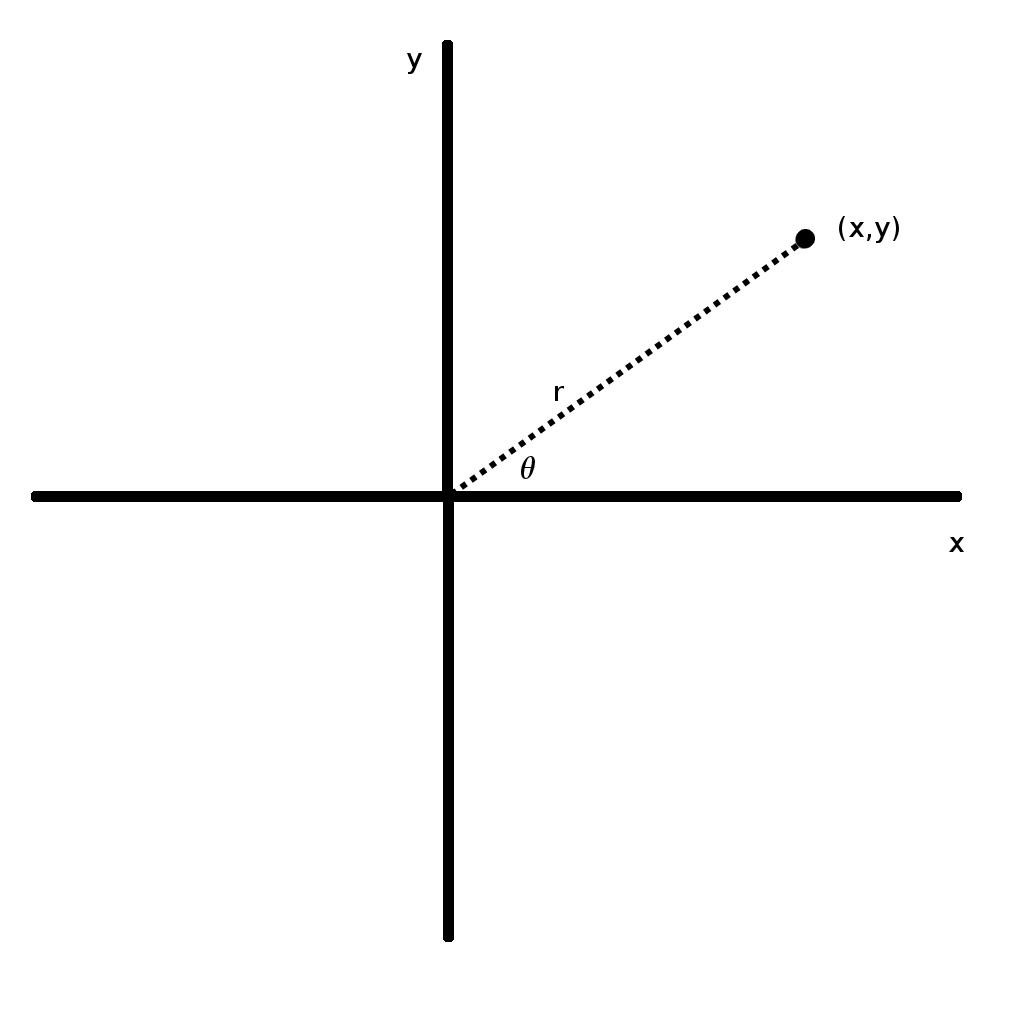
\includegraphics[height=12cm]{polar}
    \vfill


  \end{problem}
